\part{Numerical interpolation}
% \frame{\partpage}
\section{Introduction}
\subsection*{General}
\begin{frame}[label=contents_interpolation]
  \frametitle{Today's outline}
  \mode<beamer>{
    \only<1>{\tableofcontents}
  }
  \only<2>{\tableofcontents[currentsection,currentsubsection]}
\end{frame}

\begin{frame}
  \frametitle{Interpolation problem}
  \begin{definition}
  Given a set of points $x_k$, $k=0,\ldots,n$, $x_i \neq x_j$ with associated function values $f_k$, $k=0,\ldots,n$, or simply: $\{x_k,f_k\}_{k=0}^n$. The interpolation problem is defined as: find a polynomial $p_n$ such that this interpolates the values of $f_k$ on the points $x_k$:
  \[
    p_n(x_k)=f_k, \quad k=0,\ldots,n
  \]
  \end{definition}
  \pause
  \begin{theorem}
    The interpolation problem for $\{x_k,f_k\}_{k=0}^n$ has a unique solution when $x_i \neq x_j$ for $i \neq j$. Note that we cannot allow multiple function values $f_k$ for the same value of $x_k$.
  \end{theorem}
\end{frame}

\frame{
  \frametitle{What is interpolation?}
  \vfill
  \tikz{\node[emphblock,text width=\textwidth] 
    {
    Interpolation means constructing additional data points within the range of, and using, a discrete set of known data points.
    \vskip1em
    It is typically performed on a uniformly spread data set, but this is not strictly necessary for all methods
    };}
  \vfill
}
\frame{
\frametitle{Is interpolation the same as curve fitting?}
\pause
\vfill
{\begin{center} \huge NO \end{center}}
\pause
\vfill
\begin{itemize}
  \colorize<3> \item Curve-fitting requires additionally some way of computing the error between function (curve) and data
  \colorize<4> \item Curve-fitting does not strictly enforce the function to match the data exactly
  \colorize<5> \item Curve-fitting may be done on multiple datapoints at one position
  \colorize<6> \item Curve-fitting is much more expensive to do, requires optimisation
\end{itemize}
\vfill
}

\begin{frame}
  \frametitle{Why do chemical engineers need interpolation?}
  \begin{itemize}
    \colorize<1> \item Comparison of two data sets which are given at different positions
    \begin{itemize}
     \colorize<1> \item An experimental data set may have been recorded at a constant rate, but the numerical solution is computed at irregular intervals
    \end{itemize}
    \colorize<2> \item Reconstruction of field values distant of computing nodes
    \begin{itemize}
      \colorize<2> \item A CFD simulation on a regular grid containing structures that are not grid-conformant requires interpolation to the structures
    \end{itemize}
    \colorize<3> \item Calculation of a physical property at a condition between those of a lookup table
    \begin{itemize}
      \colorize<3> \item The viscosity of a substance may have been measured at 20\si{\celsius} and 30\si{\celsius}, but not at the desired 28.5\si{\celsius}
    \end{itemize}
  \end{itemize}
\end{frame}

%'exp(-x)+8*sin(x)+2*x'

\frame{
  \frametitle{General}
  Several important numerical interpolation methods are discussed today:
  \vskip2em
  \begin{itemize}
  \item Piecewise constant interpolation
  \item Linear interpolation
  \begin{itemize}
    \item Bilinear interpolation
  \end{itemize}
  \item Polynomial interpolation (Newton's method)
  \item Spline interpolation
  \end{itemize}
}

\section{Piecewise constant}
\subsection*{}
\againframe<2>{contents_interpolation}
\begin{frame}
  \frametitle{Today's data set}
  \footnotesize\selectfont
  \begin{columns}
    \column{0.45\textwidth}
    Download the datafile \lstinline$interpolation-dataset.txt$, which contains multiple data sets.\vskip2em\pause
    \begin{center}
      We start with \lstinline$x1$ and \lstinline$y1$:\vskip1em
      \begin{tabular}{c|r}
	$x_k$ & $f_k$ \\ \hline
	$0$ & $1.00$ \\
	$1$ & $\frac{11}{3}=3.67$ \\
	$2$ & $\frac{8}{3}=2.67$  \\
	$3$ & $1.00$ \\
	$4$ & $\frac{5}{3}=1.67$  \\
	$5$ & $\frac{23}{3}=7.67$ \\ \hline
      \end{tabular}
    \end{center}
    \column{0.55\textwidth}
    Data set $f_n(x_n)$ represented by \tikz{\node[interp]{};} at discrete intervals $x_n\in\{0,5\}$
    \vskip1em
    \centering
    \begin{tikzpicture}[domain=-1:6]
        \draw[gridline,step=1] (0,0) grid (5,5);
  \coordinate (O) at (0,0);
  % Axes
  \draw[line,->] (-0.3,0) -- (5,0) coordinate[label = {below:$x$}] (xmax);
  \draw[line,->] (0,-0.3) -- (0,5) coordinate[label = {left:$f(x)$}] (ymax);
  
  % Labels
  \draw (0,0) node[below left]{$0$};
  \foreach \s in {1,...,4}
  {
    \draw (\s,0) node[below]{$\s$};
    \draw (0,\s) node[left]{$\s$};
    }
    
    % Title
    %       \draw (2.5,5) node[above]{$f(x)=\frac{x^3}{2}-\frac{10x^2}{3}+\frac{11x}{2}+1$};
    
    % Plots
    \node[interp] (x0) at (0,1) {};
    \node[interp] (x1) at (1,3.667) {};
    \node[interp] (x2) at (2,2.667) {};
    \node[interp] (x3) at (3,1) {};
    \node[interp] (x4) at (4,1.667) {};
    \node (bb) at (5,5.3) {};
%       \draw [graph,domain=0:4.69] plot (\x, {0.5*\x*\x*\x-(10/3)*\x*\x+5.5*\x+1});
%       \draw [graph,opacity=0.4,dashed,domain=-0.15:4.73] plot (\x, {0.5*\x*\x*\x-(10/3)*\x*\x+5.5*\x+1});

    \end{tikzpicture}
  \end{columns}
\end{frame}

\begin{frame}
  \frametitle{Piecewise constant interpolation}
  \footnotesize\selectfont
  \begin{columns}
    \column{0.45\textwidth}
%     \begin{overlayarea}{\columnwidth}{8cm}
      \begin{itemize}
	\colorize<2> \item Nearest-neighbor interpolation in the continuous range $x\in\left[0,5\right]$
	\colorize<3> \item How to treat the point halfway (e.g. at $x=2.5$)?
% 	\hspace*{-2em}
	\begin{flalign*}
	  x \in &[0, 0.5] &\rightarrow f(x) = f(0) & \\
	  x \in &[0.5, 1.5] &\rightarrow f(x) = f(1) & \\
	  x \in &[1.5, 2.5] &\rightarrow f(x) = f(2) & \\
	  x \in &[2.5, 3.5] &\rightarrow f(x) = f(3) & \\
	  x \in &[3.5, 4.5] &\rightarrow f(x) = f(4) &
	\end{flalign*}
	\vspace*{-1em}
	\colorize<4> \item Not often used for simple problems, but e.g. for 2D (Voronoi)
      \end{itemize}
%     \end{overlayarea}
    \column{0.55\textwidth}
    Data set $f_n(x_n)$ represented by \tikz{\node[interp]{};} at discrete intervals $x_n\in\{0,5\}$
    \vskip1em
    \centering
    \begin{tikzpicture}[domain=-1:6]
        \draw[gridline,step=1] (0,0) grid (5,5);
  \coordinate (O) at (0,0);
  % Axes
  \draw[line,->] (-0.3,0) -- (5,0) coordinate[label = {below:$x$}] (xmax);
  \draw[line,->] (0,-0.3) -- (0,5) coordinate[label = {left:$f(x)$}] (ymax);
  
  % Labels
  \draw (0,0) node[below left]{$0$};
  \foreach \s in {1,...,4}
  {
    \draw (\s,0) node[below]{$\s$};
    \draw (0,\s) node[left]{$\s$};
    }
    
    % Title
    %       \draw (2.5,5) node[above]{$f(x)=\frac{x^3}{2}-\frac{10x^2}{3}+\frac{11x}{2}+1$};
    
    % Plots
    \node[interp] (x0) at (0,1) {};
    \node[interp] (x1) at (1,3.667) {};
    \node[interp] (x2) at (2,2.667) {};
    \node[interp] (x3) at (3,1) {};
    \node[interp] (x4) at (4,1.667) {};
    \node (bb) at (5,5.3) {};
%       \draw [graph,domain=0:4.69] plot (\x, {0.5*\x*\x*\x-(10/3)*\x*\x+5.5*\x+1});
%       \draw [graph,opacity=0.4,dashed,domain=-0.15:4.73] plot (\x, {0.5*\x*\x*\x-(10/3)*\x*\x+5.5*\x+1});


      % Piecewise interpolant
      \draw<2->[interp] (0,1) -- (0.5,1);
      \draw<2->[interp] (0.5,3.667) -- (1.5,3.667);
      \draw<2->[interp] (1.5,2.667) -- (2.5,2.667);
      \draw<2->[interp] (2.5,1)     -- (3.5,1);
      \draw<2->[interp] (3.5,1.667) -- (4.5,1.667);
    \end{tikzpicture}
  \end{columns}
\end{frame}

\section{Linear}
\subsection*{}
\againframe<2>{contents_interpolation}
\begin{frame}
  \frametitle{Linear interpolation}
  \footnotesize\selectfont
  \begin{columns}
    \column{0.45\textwidth}
    \begin{itemize}
      \colorize<2> \item Linear interpolation to $(x,y)$ between 2 data points $(x_2,y_2)$ and $(x_3,y_3)$:
      \colorize<3> {\[ {\color<3>{tuegreen}\frac{y-y_2}{x-x_2}}=\color<3>{tuered}\frac{y_3-y_2}{x_3-x_2} \] }
      \colorize<4> \item Reordered, and more formally: 
      \[ y = y_n + (y_{n+1} - y_n)\frac{x-x_n}{x_{n+1}-x_n} \]
    \end{itemize}
    \column{0.55\textwidth}
    Data set $f_n(x_n)$ represented by \tikz{\node[interp]{};} at discrete intervals $x_n\in\{0,5\}$
    \vskip1em
    \centering
    \begin{tikzpicture}[domain=-1:6]
        \draw[gridline,step=1] (0,0) grid (5,5);
  \coordinate (O) at (0,0);
  % Axes
  \draw[line,->] (-0.3,0) -- (5,0) coordinate[label = {below:$x$}] (xmax);
  \draw[line,->] (0,-0.3) -- (0,5) coordinate[label = {left:$f(x)$}] (ymax);
  
  % Labels
  \draw (0,0) node[below left]{$0$};
  \foreach \s in {1,...,4}
  {
    \draw (\s,0) node[below]{$\s$};
    \draw (0,\s) node[left]{$\s$};
    }
    
    % Title
    %       \draw (2.5,5) node[above]{$f(x)=\frac{x^3}{2}-\frac{10x^2}{3}+\frac{11x}{2}+1$};
    
    % Plots
    \node[interp] (x0) at (0,1) {};
    \node[interp] (x1) at (1,3.667) {};
    \node[interp] (x2) at (2,2.667) {};
    \node[interp] (x3) at (3,1) {};
    \node[interp] (x4) at (4,1.667) {};
    \node (bb) at (5,5.3) {};
%       \draw [graph,domain=0:4.69] plot (\x, {0.5*\x*\x*\x-(10/3)*\x*\x+5.5*\x+1});
%       \draw [graph,opacity=0.4,dashed,domain=-0.15:4.73] plot (\x, {0.5*\x*\x*\x-(10/3)*\x*\x+5.5*\x+1});

      
      % Interpolant points and captions
      \draw<2->[dot,draw=none] (x2) -- node[interp,color=tuered,midway,fill=white] (xy){} (x3);
      \node<2->[anchor=north east] at (xy.west) {$(x,y)$};
      \node<2->[anchor=south west] at (x2.east) {$(x_2,y_2)$};
      \node<2->[anchor=south west] at (x3.east) {$(x_3,y_3)$};
      % Slopes between the points in colors
      \draw<3>[dot,draw=tuegreen,line width=3pt] (x2) -- (xy);
      \draw<3->[dot] (x2) -- node[interp,color=tuered,midway,fill=white] (xy){} (x3);

      % Linear interpolant
      \draw<4->[interp] (0,1) node[interp]{} -- (1,3.667) node[interp]{} -- (2,2.667) node[interp]{} -- (3,1) node[interp]{} -- (4,1.667) node[interp]{} -- (4.555,5);
      \draw<4->[interp,opacity=0.5] (4.555,5) --(4.61388,5.35);
      \draw<4->[interp,opacity=0.5] (0,1) -- (-0.1,0.108);
    \end{tikzpicture}
  \end{columns}
\end{frame}

\begin{frame}
  \frametitle{Linear interpolation}
  \begin{itemize}
    \colorize<1> \item While linear interpolation is fast, and relatively easy to program, it is not very accurate
    \colorize<2> \item At the nodes, the derivatives are discontinuous i.e. not differentiable
    \colorize<3> \item Error is proportional to the square of the distance between nodes
  \end{itemize}
\end{frame}

\begin{frame}[t,fragile]
  \frametitle{Example: Linear interpolation in Python}
  \footnotesize\selectfont
  Consider the data set in \lstinline$sim_exp_dataset.mat$, containing a normalized concentration and time vector for an experiment and a simulation. The simulation was performed with adaptive node distance to save computation time, thus the concentration is not known at the same times. We are not able to compare yet.
  \vfill
  \begin{tikzpicture}
    \begin{axis}[
        width=\textwidth, height=5.5cm,     % size of the image
        grid = major,
        grid style={dashed, gray!30},
        %xmode=log,log basis x=10,
        %ymode=log,log basis y=10,
        xmin=0,     % start the diagram at this x-coordinate
        xmax=200,    % end   the diagram at this x-coordinate
        ymin=0,     % start the diagram at this y-coordinate
        ymax=0.02,   % end   the diagram at this y-coordinate
        /pgfplots/xtick={0,25,...,200}, % make steps of length 5
        /pgfplots/ytick={0.005,0.01,...,0.02}, % make steps of length 5
        axis background/.style={fill=white},
        ylabel=Concentration (\si{\mol\per\cubic\meter}),
        xlabel=Time (\si{\second}),
        tick align=outside,
        legend style={draw=none,fill=none}]

      % import the correct data from a CSV file
      \addplot[draw=tuered,mark=*,mark options={fill=white},mark size=0.7pt] table [id=exp]{student-data/exp_data.txt};
      \addlegendentry{Experiment};
      \addplot[draw=tueblue,mark=triangle*,mark options={fill=white},mark size=0.7pt] table [id=sim]{student-data/sim_data.txt};
      \addlegendentry{Simulation};
      % plot the stirling-formulae
%       \addplot[domain=0:60, red, thick] {1-(365/(365-x))^(365.5-x)*e^(-x)}; 
    \end{axis} 
\end{tikzpicture}
\end{frame}

\begin{frame}[t,fragile]
  \frametitle{Example: Linear interpolation in Python}
  \footnotesize\selectfont
  Consider the data set in \lstinline$sim_dataset.txt$ and \lstinline$exp_dataset.txt$, containing a normalized concentration and time vector for an experiment and a simulation. The simulation was performed with adaptive node distance to save computation time, thus the concentration is not known at the same times. We are not able to compare yet.
  \vfill
 \begin{columns}
  \column{0.49\textwidth}
  \begin{lstlisting}[language=Python,basicstyle=\tiny]
import numpy as np
import matplotlib.pyplot as plt

t_sim, c_sim = np.loadtxt("./student-data/sim_data.txt").T
t_exp, c_exp = np.loadtxt("./student-data/exp_data.txt").T

# Linear interpolation
c_sim_new = np.interp(t_exp, t_sim, c_sim)
diff = np.abs(c_exp - c_sim_new)

# Plot the solution
plt.subplot(2, 1, 1)
plt.plot(t_exp, c_exp, 'b-x', label='c_exp')
plt.plot(t_exp, c_sim_new, 'r-o', label='c_sim_new')
plt.legend()

plt.subplot(2, 1, 2)
plt.plot(t_exp, diff); plt.show()

# Compute the L2-norm
norm = np.linalg.norm(diff)
print(norm)
  \end{lstlisting}
  \column{0.5\textwidth}
  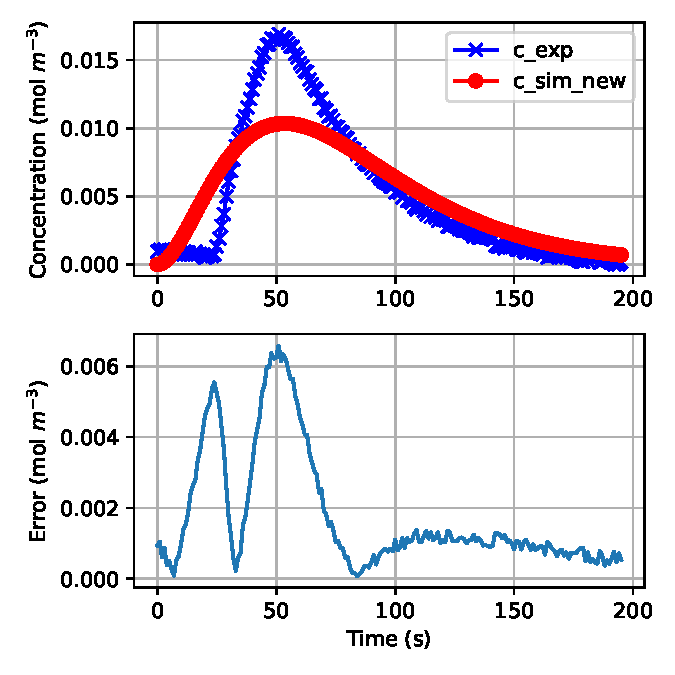
\includegraphics[width=0.8\textwidth]{sim_exp_data_interp.pdf}
\end{columns}
\end{frame}



\begin{frame}
  \frametitle{Bi-linear interpolation}
  When a 2D field of some quantity is known, we can interpolate the solution to an arbitrary position in the 2D domain $p(x,y)$ using 4 field values $f_{00}$, $f_{10}$, $f_{01}$ and $f_{11}$.
  \begin{columns}
    \column{0.5\textwidth}
      \colorize<3> 
      \begin{align*}
	g_1 &= f_{01}\frac{x_1-x}{x_1-x_0} + f_{11}\frac{x-x_0}{x_1-x_0} \\
	    &= f_{01}\frac{x_1-x}{\Delta x} + f_{11}\frac{x-x_0}{\Delta x}
      \end{align*}
      \colorize<4> 
      \[
	g_2 = f_{00}\frac{x_1-x}{\Delta x} + f_{10}\frac{x-x_0}{\Delta x}
      \]
      \colorize<5> 
      \[
	p = g_2\frac{y_1-y}{\Delta y} + g_1\frac{y-y_0}{\Delta y}
      \]
    \column{0.5\textwidth}
      \begin{tikzpicture}[scale=2.5]
	\draw[line,-,step=1] (0,0) grid (1,1);
	\coordinate (O) at (0,0);
	\node[interp,fill=tueblue] (x0) at (0,0) {};
	\node[interp,fill=tueblue] (x1) at (1,0) {};
	\node[interp,fill=tueblue] (x2) at (1,1) {};
	\node[interp,fill=tueblue] (x3) at (0,1) {};
	\node<3->[interp,draw=tuegreen,fill=tuegreen] (g1) at (0.75,1) {};
	\node<4->[interp,draw=tuegreen,fill=tuegreen] (g2) at (0.75,0) {};
	
	\node[interp,draw=tuered,fill=tuered] (p) at (0.75,0.6) {};
	
	\node[below=1ex of x0,anchor=north east] {$f_{00}=4.0$};
	\node[below=1ex of x1,anchor=north west] {$f_{10}=6.0$};
	\node[above=1ex of x2,anchor=south west] {$f_{11}=1.0$};
	\node[above=1ex of x3,anchor=south east] {$f_{01}=8.0$};
	\node[right=-0.3ex of p] {$p$};
	\node<3->[above=1ex of g1] {$g_1$};
	\node<4->[below=1ex of g2] {$g_2$};
	\draw<2>[line,dashed,gray] (x0)--(p);
	\draw<2>[line,dashed,gray] (x1)--(p);
	\draw<2>[line,dashed,gray] (x2)--(p);
	\draw<2>[line,dashed,gray] (x3)--(p);
	\draw<5->[line,-,dashed,gray] (g1)--(g2);
	
	\draw[line,stealth'-stealth'] ($(x0)+(0,0.1)$) -- node[midway,above]{$\Delta x$}($(x1)+(0,0.1)$);
	\draw[line,stealth'-stealth'] ($(x0)+(0.1,0)$) -- node[midway,right]{$\Delta y$}($(x3)+(0.1,0)$);
      \end{tikzpicture}
  \end{columns}
  \onslide<6>{ \vskip1em
  \begin{itemize}
    \item The order of interpolation ($x$ or $y$ direction first) does not matter; the results are equal
  \end{itemize}
  }
\end{frame}

\begin{frame}
  \frametitle{Higher-dimensional field interpolation in Python}
  2D or higher-dimensional fields of data can be interpolated in Python using the \lstinline$scipy.interpolate.interp2d$, \lstinline$scipy.interpolate.interp3d$, or even \lstinline$scipy.interpolate.RegularGridInterpolator$ functions. The method can be adjusted:
  \vskip1em
  \begin{columns}
    \column{0.33\textwidth}
      \centering
      \lstinline$'nearest'$
      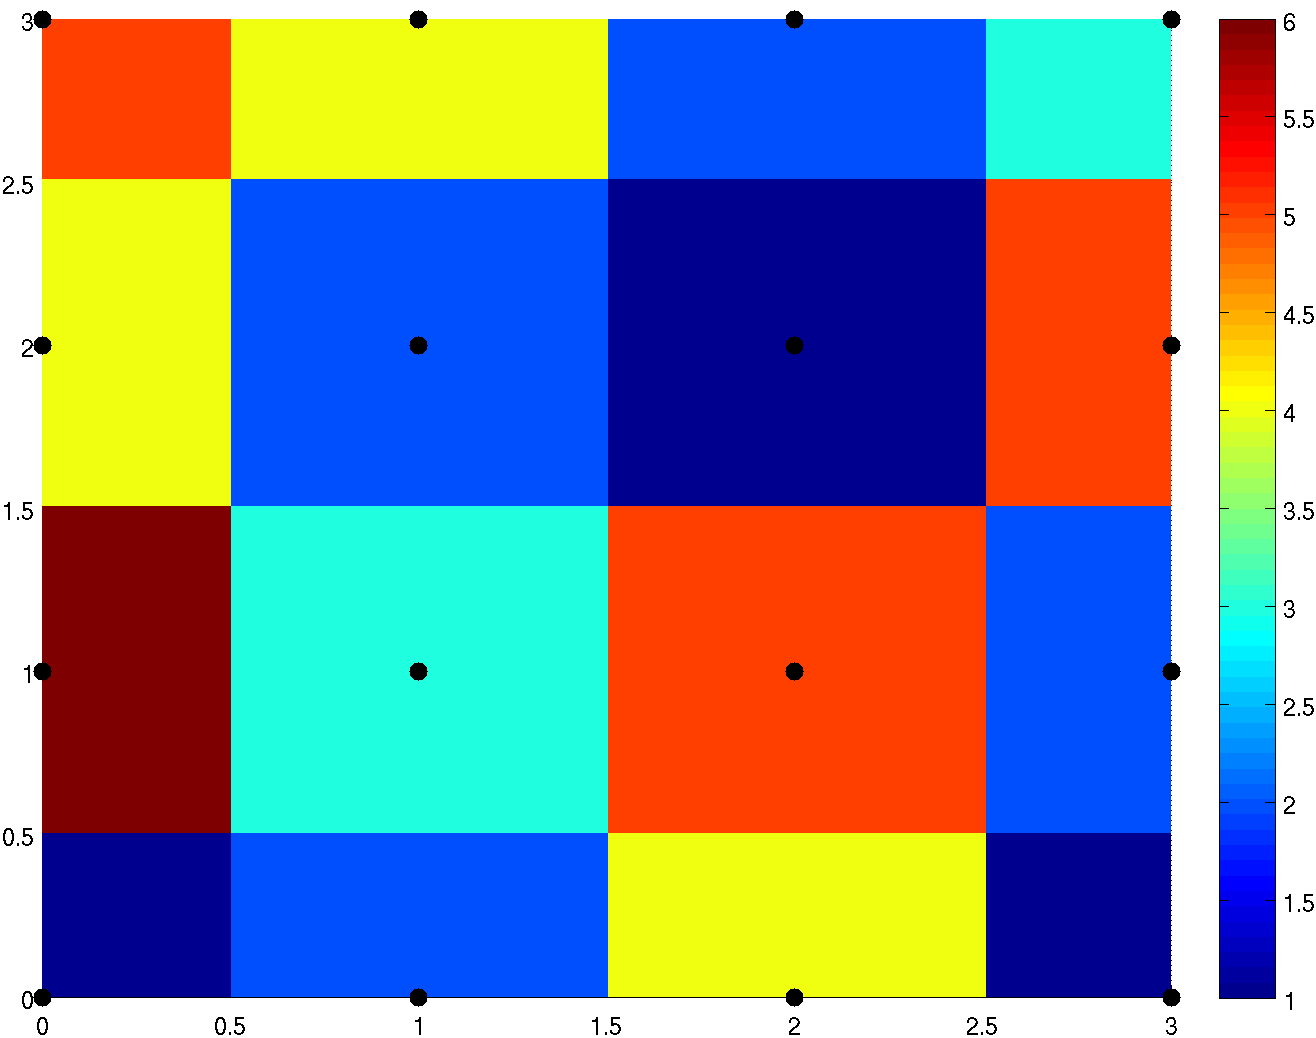
\includegraphics[width=\columnwidth]{Nearest2DInterpolExample.png}
    \column{0.33\textwidth}
      \centering
      \lstinline$'linear'$
      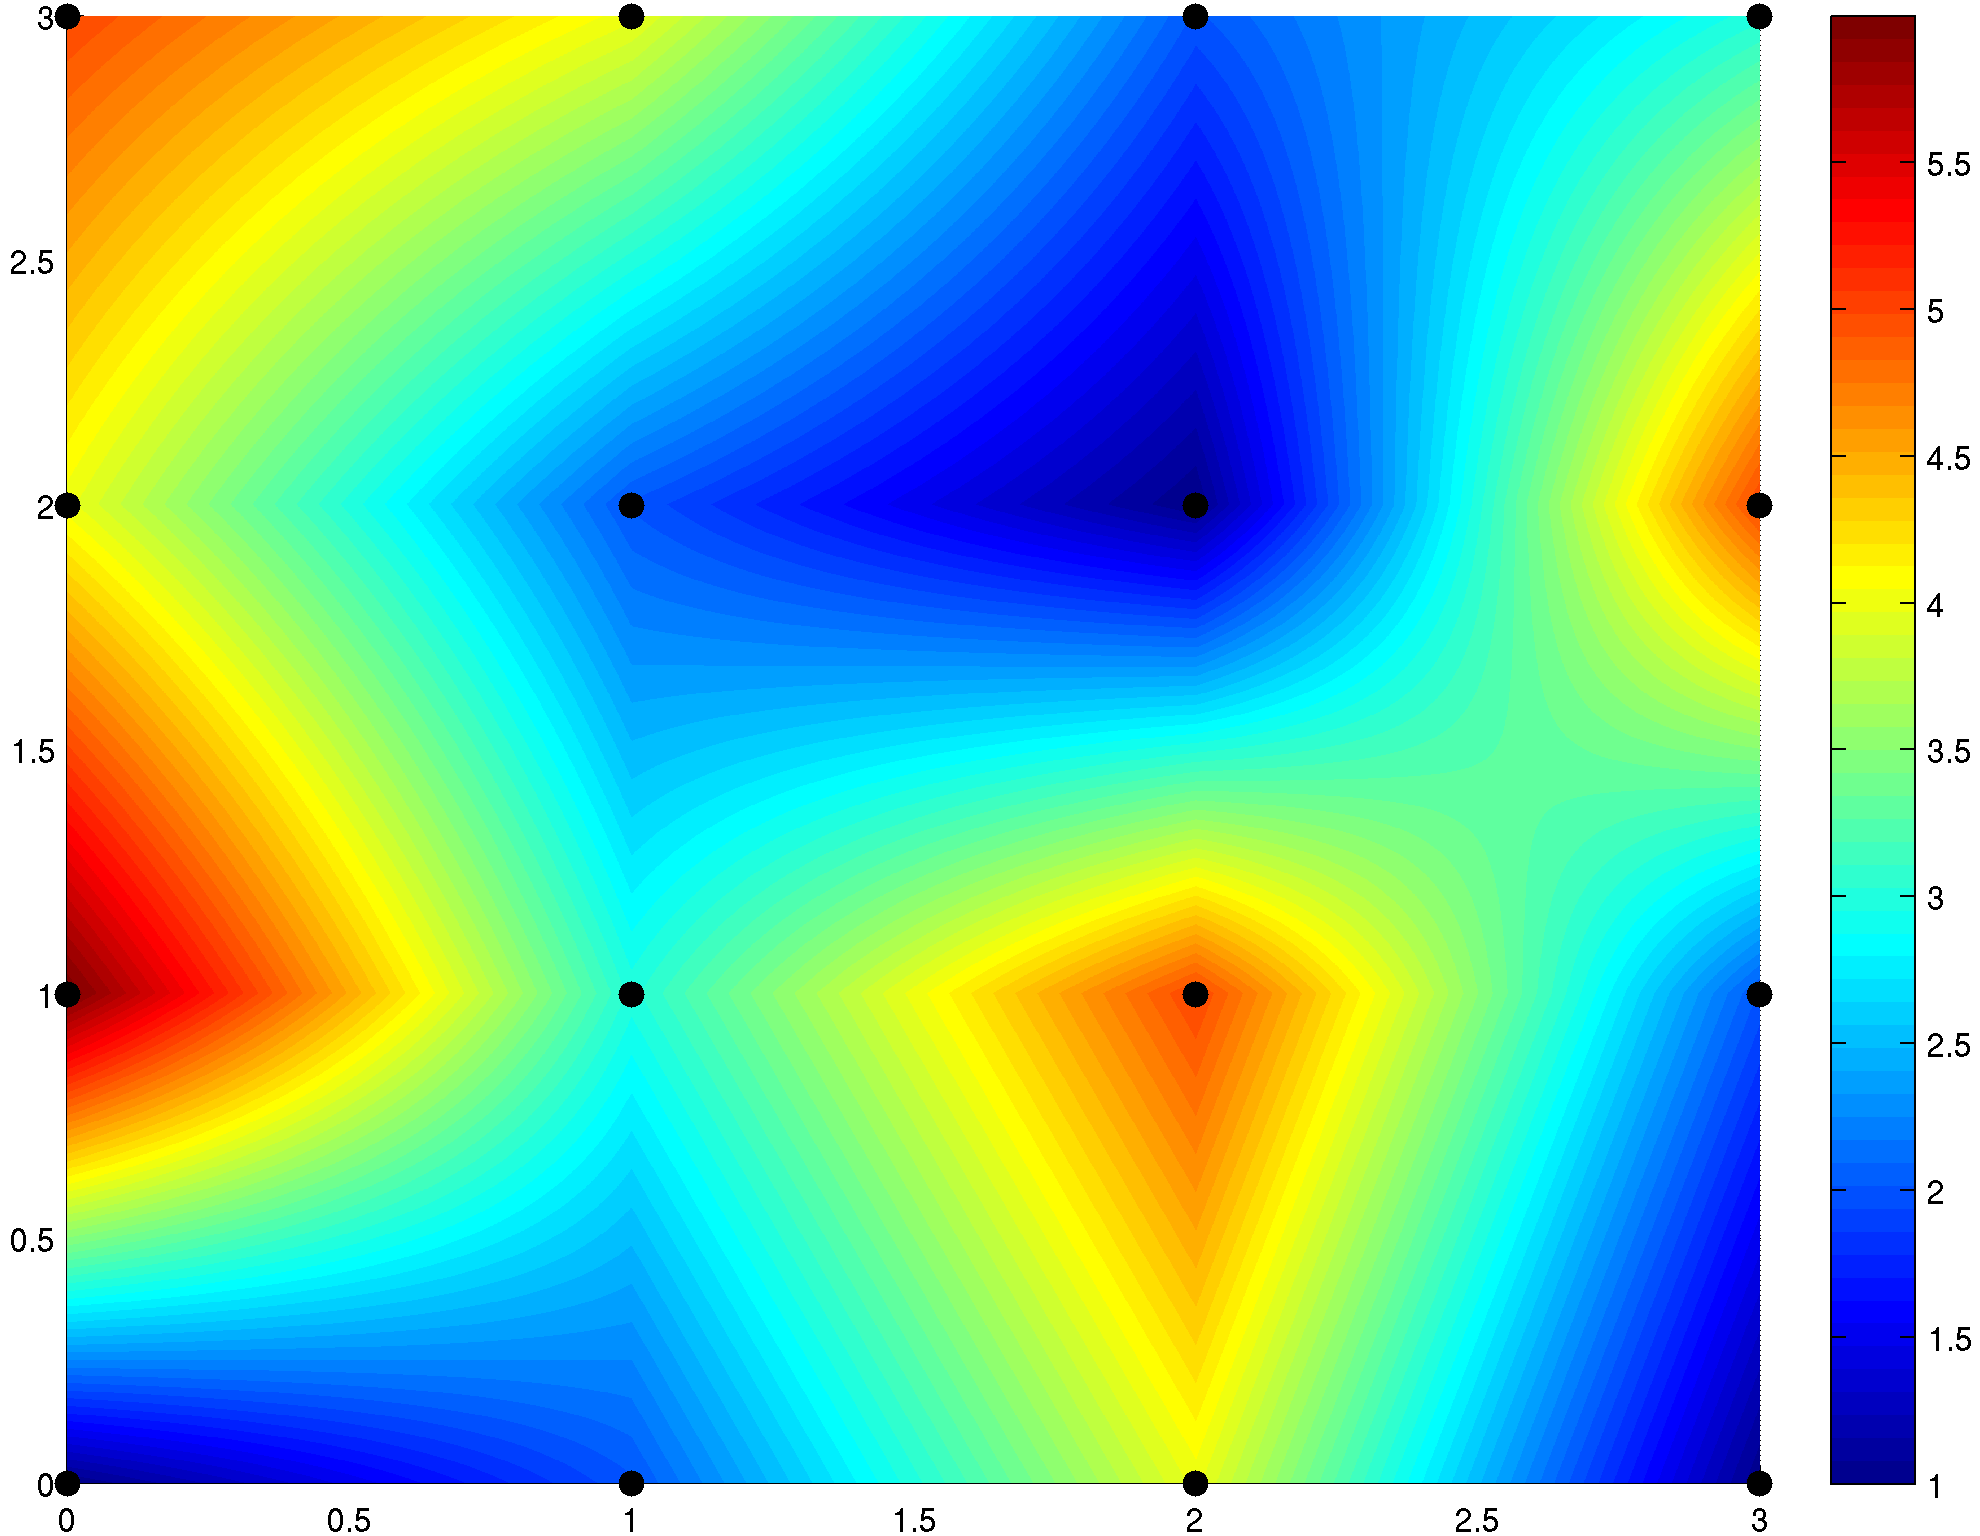
\includegraphics[width=\columnwidth]{BilinearInterpolExample.png}
    \column{0.33\textwidth}
      \centering
      \lstinline$'cubic'$
      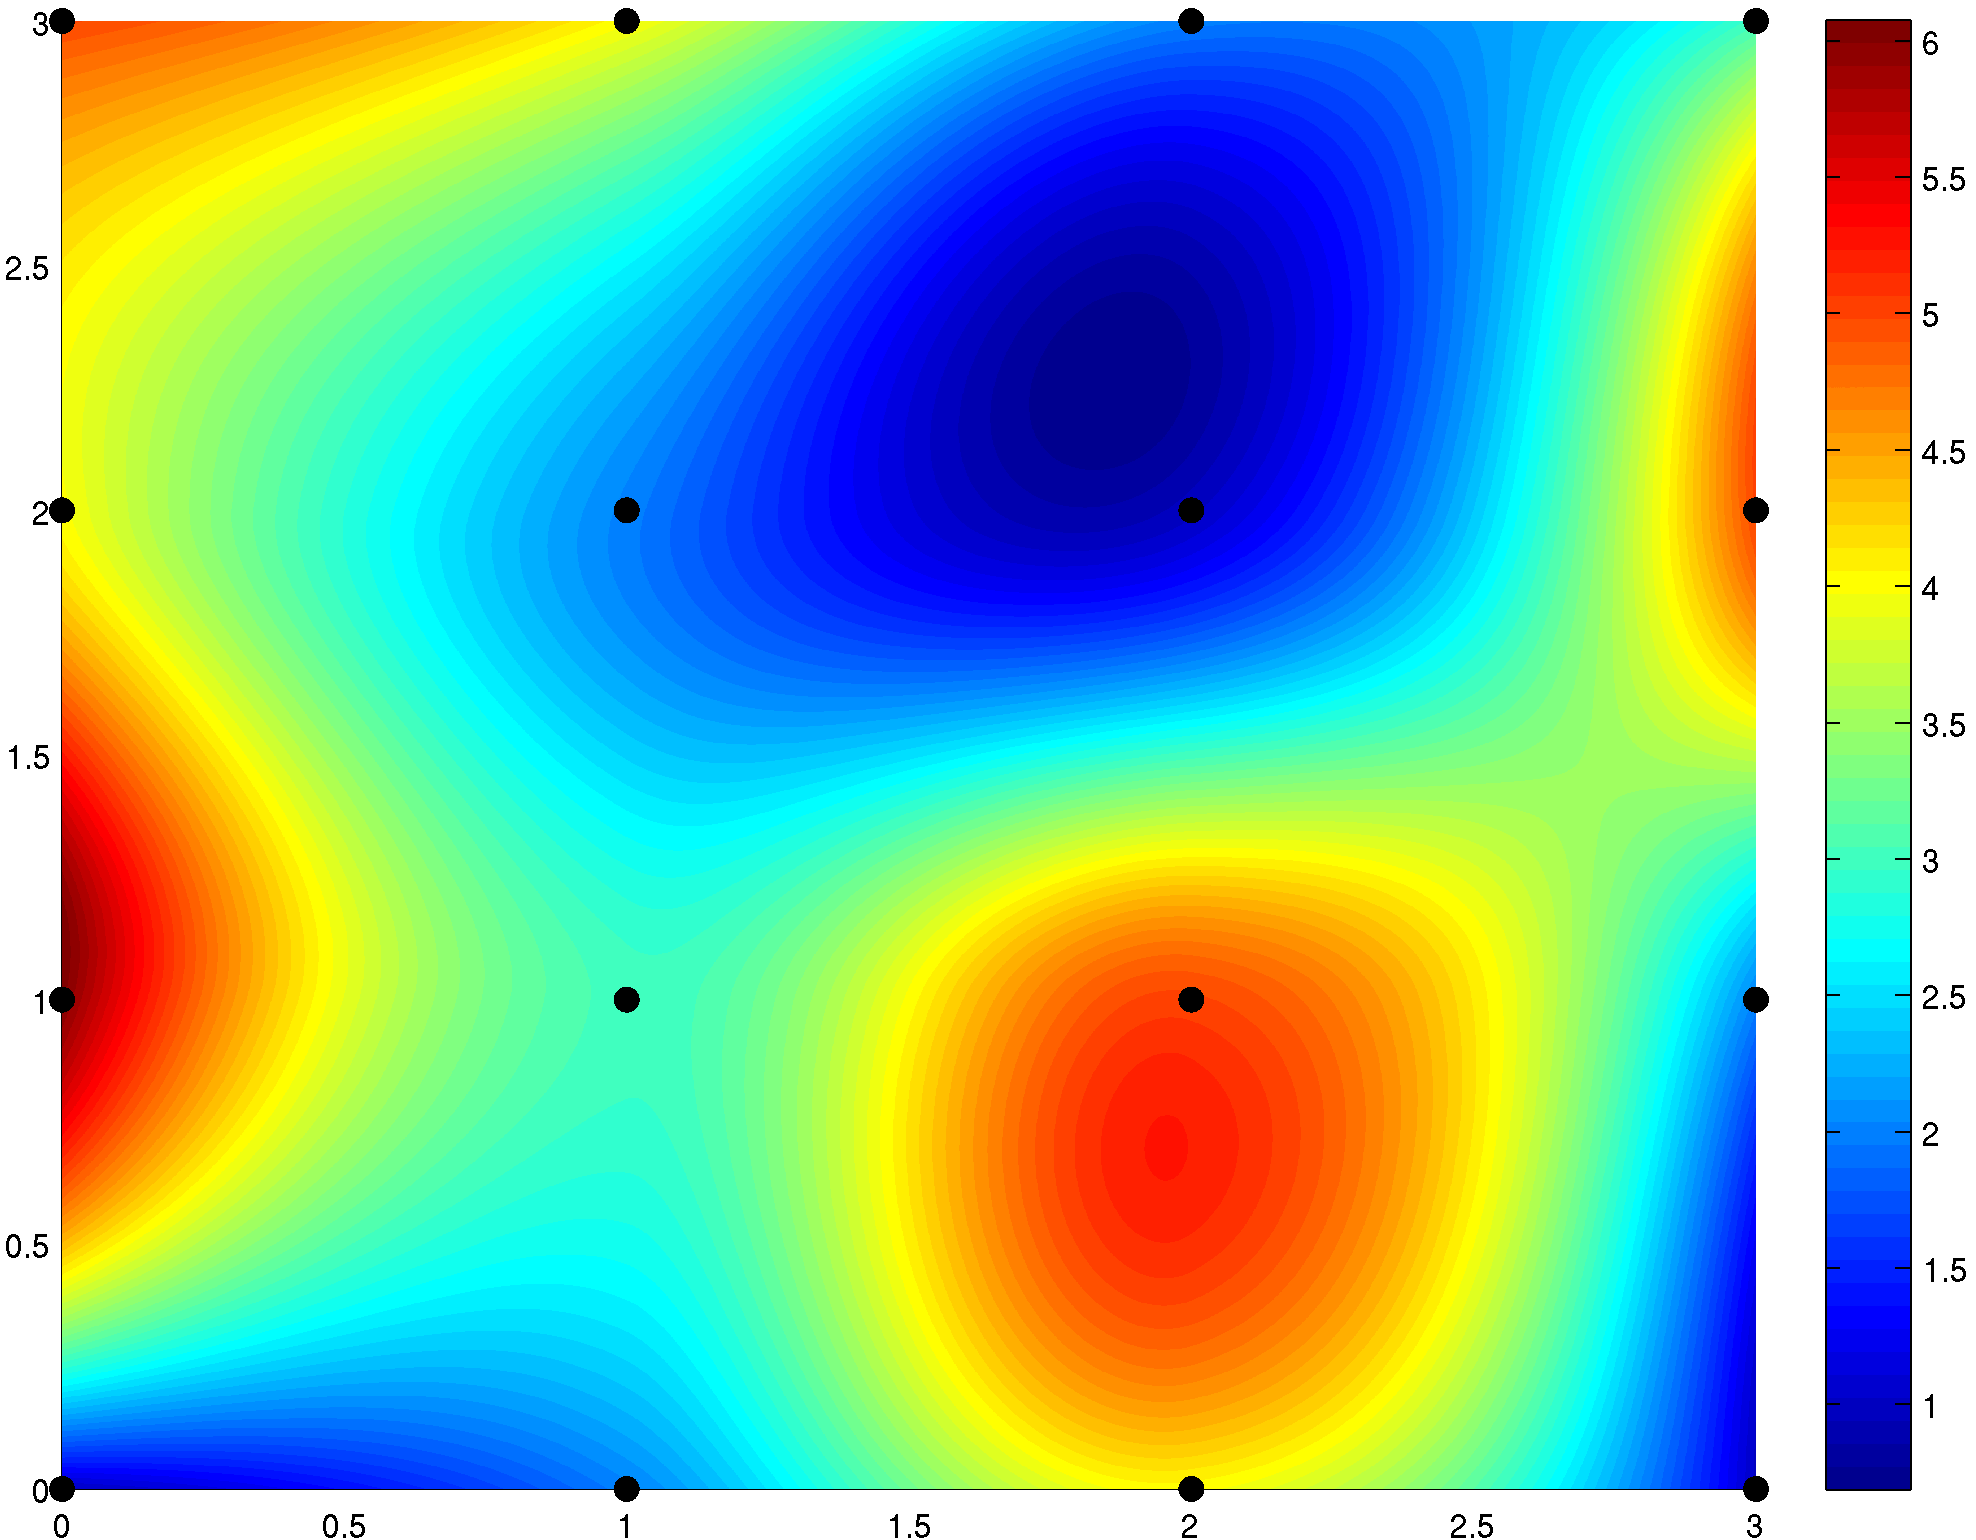
\includegraphics[width=\columnwidth]{BicubicInterpolationExample.png}
  \end{columns}
  \vskip1em
  \begin{itemize}
    \item Similar to 1D linear interpolation, the derivatives are discontinuous on the grid nodes.
    \item Also consider tri-linear interpolation (for 3D fields) with \lstinline$scipy.interpolate.LinearNDInterpolator$, or bicubic interpolation (2D, but third order) with \lstinline$scipy.interpolate.interp2d$.
  \end{itemize}
\end{frame}


\begin{frame}
  \frametitle{A practical example}
  Field interpolation is used in e.g. CFD simulations, e.g. a fluidized bed simulation using a \emph{discrete particle model}, where particles are found in between the grid nodes used for velocity computation.\\
  \centering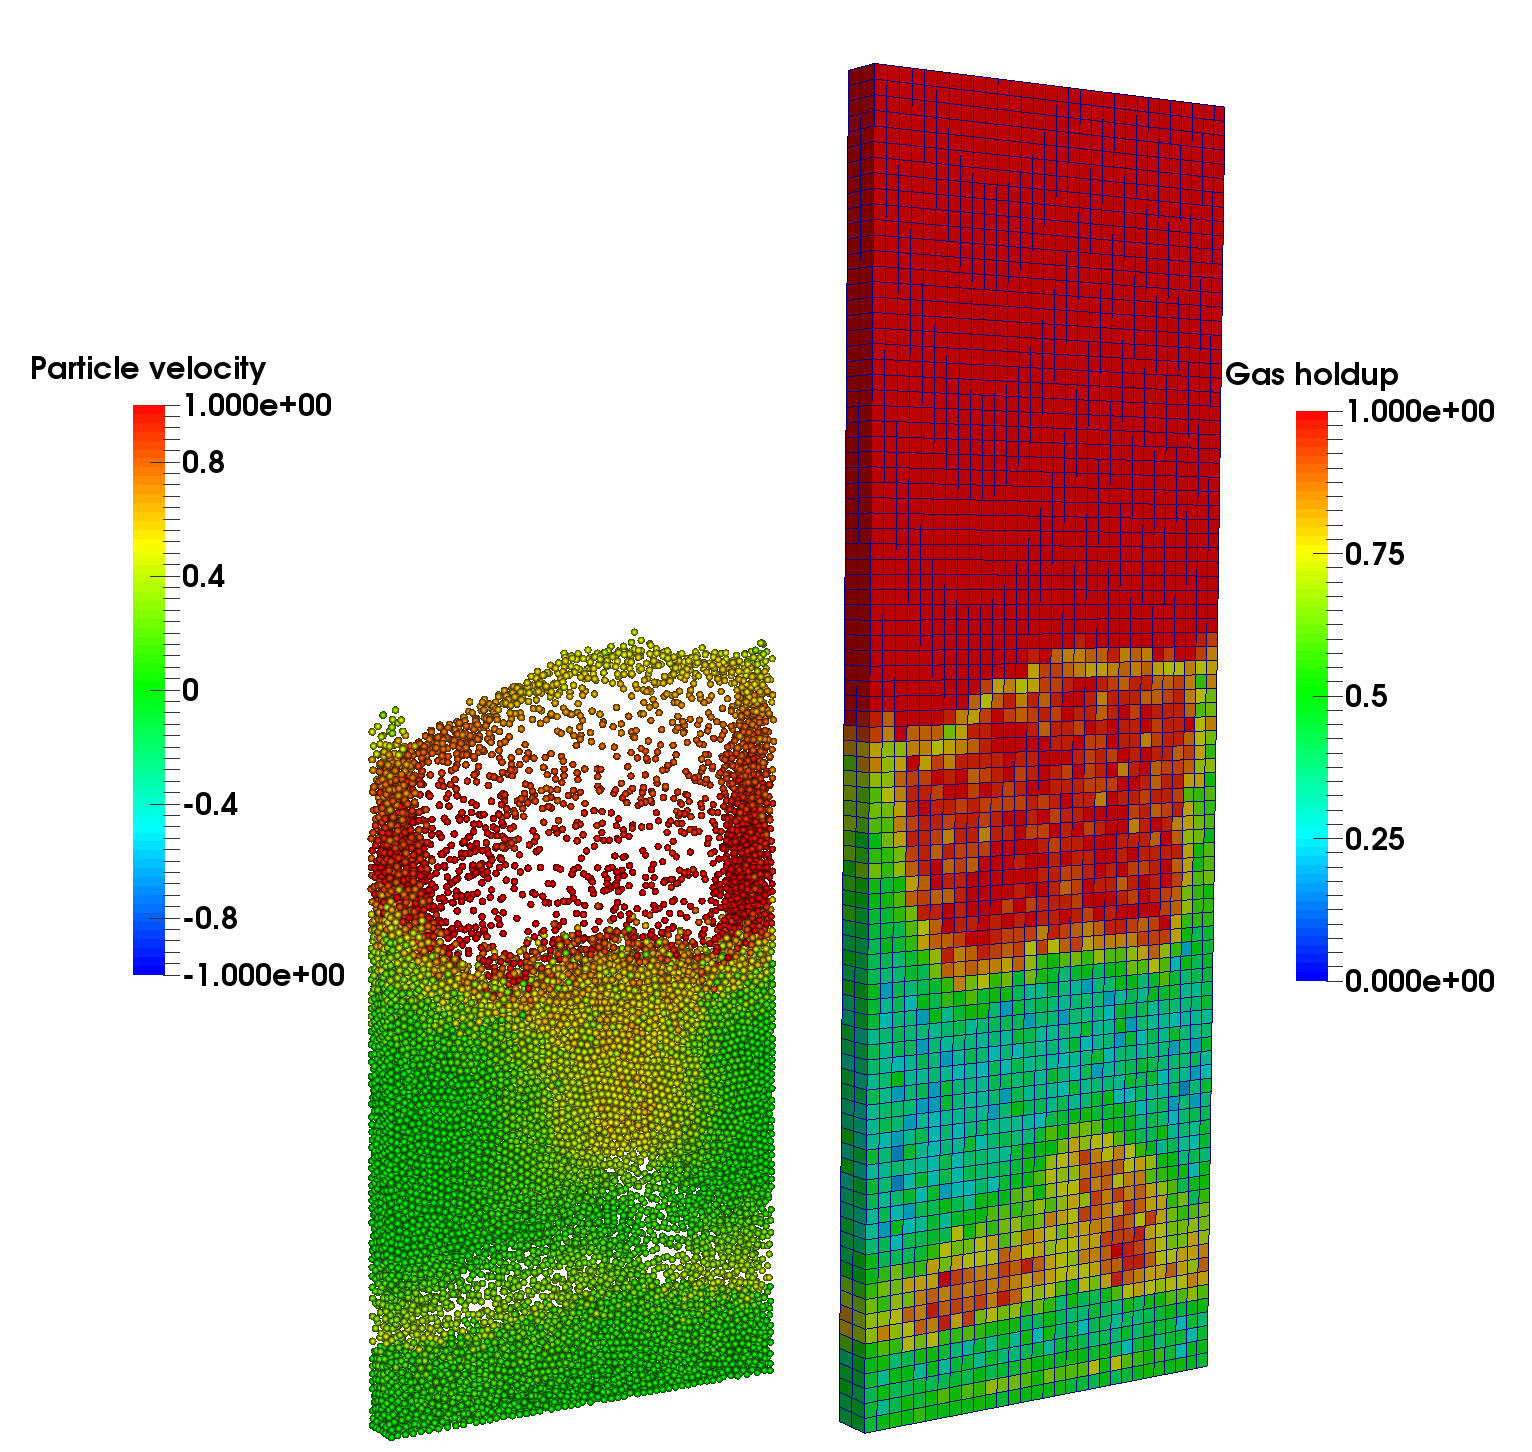
\includegraphics[width=0.4\textwidth]{fluidbed}
\end{frame}

\section{Polynomial}
\subsection*{}
\againframe<2>{contents_interpolation}
\begin{frame}
  \frametitle{Polynomial interpolation}
  The examples that we have seen, are simplified forms of \emph{Newton polynomials}. We can interpolate our data with a polynomial of degree $n$:
  
  \vskip2em
  \[
    p_n(x) = a_n x^n + a_{n-1}x^{n-1} + \ldots + a_2x^2 + a_1 x + a_0
  \]

\end{frame}

\begin{frame}[fragile]
  \frametitle{Polynomial interpolation via Vandermonde matrix}
  \footnotesize\selectfont
  \rowcolors[]{50}{white}{white}
  Consider the data points $(x_1,y_1),\, (x_2,y_2),\, \ldots,\,(x_m,y_m)$, the Vandermonde matrix $V$, coefficient vector $a$ and function value vector $y$: \vskip1em
  $V_{m,n} =
 \begin{pmatrix}
  x_1^0 & x_1^1 & x_1^2 & \cdots & x_1^{n-1} \\
  x_2^0 & x_2^1 & x_2^2 & \cdots & x_2^{n-1} \\
  \vdots  & \vdots & \vdots & \ddots & \vdots  \\
  x_m^0 & x_m^1 & x_m^2 & \cdots & x_m^{n-1}
 \end{pmatrix} \quad  
 a=
 \begin{pmatrix}
   a_0 \\
   a_1 \\
   \vdots\\
   a_{n-1}
 \end{pmatrix} \quad
 y=
 \begin{pmatrix}
   y_1 \\
   y_2 \\
   \vdots\\
   y_m
 \end{pmatrix}
$\vskip1em
The coefficients of a polynomial through the data points can be obtained by solving the linear system $Va=y$.
\pause
\begin{columns}
  \column{0.5\textwidth}
    \begin{lstlisting}[language=Python]
import numpy as np
x = np.array([0, 1, 2])
y = np.array([1.0000, 3.6667, 2.6667])
V = np.vander(x, increasing=True)
a = np.linalg.solve(V, y)
print(a)
# Output
# [-1.8333, 4.5000, 1.0000]
    \end{lstlisting}
  \column{0.5\textwidth}
  \pause
  So we found the equation:
  \[
    p_2(x) = -1.8333 x^2 + 4.5x - 1
  \]
  \pause
  \tikz{\node[emphblock,text width=\columnwidth] {These Vandermonde-systems are often \emph{ill-conditioned}, so we need another, more stable, method!
};}
\end{columns}
\end{frame}


\begin{frame}
  \frametitle{Construction of Newton polynomials}
  \footnotesize\selectfont
  Formally, the polynomials $p_n(x)$ are described using prefactors $f[x_0,\ldots,x_k]$ and polynomial terms $w_m(x)$:
  \[
    p_n(x) = \sum_{k=0}^n f[x_0,\ldots,x_k] w_k(x)
  \]
  \pause
  The polynomial terms are computed via:
  \begin{align*}
    &w_0(x) = 1, \ w_1(x)=(x-x_0), \ w_2(x)=(x-x_0)\cdot(x-x_1), \\
    &w_m(x)=(x-x_0)\cdot(x-x_1)\cdots(x-x_{m-1}) = w_{m-1}\cdot(x-x_{m-1})\\
    &w_m(x) = \prod_{j=0}^{m-1} (x-x_j), \qquad m=0,\ldots,n
  \end{align*}
  \pause
  The prefactors are \emph{forward divided differences}, which can be computed as:
    \[
      f[x_{x-k},\ldots,x_r] \equiv \frac{f[x_{r-k+1},\ldots,x_r]-f[x_{r-k},\ldots,x_{r-1}]}{x_r-x_{r-k}} 
    \]
\end{frame}

% 
%       \begin{align*}
% 	p_n(x)                &= \sum_{k=0}^n f[x_0,\ldots,x_k] w_k(x) \\
% 	w_m(x)                &= \prod_{j=0}^{m-1} (x-x_j) \\
% 	f[x_{x-k},\ldots,x_r] &\equiv \frac{f[x_{r-k+1},\ldots,x_r]-f[x_{r-k},\ldots,x_{r-1}]}{x_r-x_{r-k}} 
%       \end{align*}

\begin{frame}
  \frametitle{Construction of Newton polynomials: example}
  \footnotesize\selectfont
  \rowcolors[]{1}{maincolor!20}{maincolor!10}
  \begin{columns}[T]
    \begin{column}{0.2\textwidth}
    \centering Sample data
      \begin{longtable}{c|r}
	$x_k$ & $f_k$ \\ \hline
	$0$ & $1.00$ \\
	$1$ & $\frac{11}{3}=3.67$ \\
	$2$ & $\frac{8}{3}=2.67$ 
      \end{longtable}
    \end{column}
    \hfill
    \begin{column}{0.8\textwidth}
      \begin{tikzpicture}[myNode/.style={rectangle,draw=maincolor,fill=maincolor!20,text centered,rounded corners,thick,minimum height=2em}]
	\node[myNode] (a) {${\scriptstyle p_n(x)= \sum_{k=0}^n f[x_0,\ldots,x_k] w_k(x)}$};
	\node[myNode,below left=1.2cm of a.south west,anchor=center] (c) {${\scriptstyle f[x_{x-k},\ldots,x_r] \equiv \frac{f[x_{r-k+1},\ldots,x_r]-f[x_{r-k},\ldots,x_{r-1}]}{x_r-x_{r-k}}}$};
	\node[myNode,below right=1.2cm of a.south east,anchor=center] (b) {${\scriptstyle w_m(x) = \prod_{j=0}^{m-1} (x-x_j)}$};
	\draw[->,>=stealth] (c.north) -> (a.south west);
	\draw[->,>=stealth] (b.north) -> (a.south east);
      \end{tikzpicture}
    \end{column}
  \end{columns}
    \onslide<2->{
      \begin{longtable}{c|ccc}
	$x_k$ & $f_k$ & & \\ \hline 
	\color<2>{tuered} $x_0$ & \color<2>{tuered} $f[x_0]=f_0$ & & \onslide<3->{\\
	\color<3>{tuered} $x_1$ & \color<3>{tuered} $f[x_1]=f_1$ & \color<3>{tuered} $f[x_0,x_1]=\frac{f_1-f_0}{x_1-x_0}$& \onslide<4->{\\
	\color<4>{tuered} $x_2$ & \color<4>{tuered} $f[x_2]=f_2$ & \color<4>{tuered} $f[x_1,x_2]=\frac{f_2-f_1}{x_2-x_1}$& \color<4>{tuered} $f[x_0,x_1,x_2] = \frac{f[x_1,x_2]-f[x_0,x_1]}{x_2-x_0}$ }}
      \end{longtable}}
  \onslide<2->{
    \begin{longtable}{c|lll}
      $x_k$ & $f_k$ & & \\ \hline
      \color<2>{tuered} $0$ & \color<2>{tuered} $1$ & & \onslide<3->{\\
      \color<3>{tuered} $1$ & \color<3>{tuered} $3.67$ & \color<3>{tuered} $\frac{\frac{11}{3}-1}{1-0}=\frac{8}{3}$& \onslide<4>{\\
      \color<4>{tuered} $2$ & \color<4>{tuered} $2.67$ & \color<4>{tuered} $\frac{\frac{8}{3}-\frac{11}{3}}{2-1}=\frac{-1}{1}=-1$& \color<4>{tuered} $\frac{(-1)-\frac{8}{3}}{2-0}=-\frac{11}{6}$ }}
    \end{longtable}
  }
\end{frame}

\begin{frame}
  \frametitle{Construction of Newton polynomials: example}
  \footnotesize\selectfont
  \rowcolors[]{1}{maincolor!20}{maincolor!10}
  \begin{columns}[T]
    \begin{column}{0.2\textwidth}
    \centering Sample data
      \begin{longtable}{c|r}
	$x_k$ & $f_k$ \\ \hline
	{\color<4->{tuedyellow}$0$} & $1.00$ \\
	{\color<4->{tuepurple}$1$} & $\frac{11}{3}=3.67$ \\
	$2$ & $\frac{8}{3}=2.67$ 
      \end{longtable}
    \end{column}
    \hfill
    \begin{column}{0.8\textwidth}
      \begin{tikzpicture}[myNode/.style={rectangle,draw=maincolor,fill=maincolor!20,text centered,rounded corners,thick,minimum height=2em}]
	\node[myNode] (a) {${\scriptstyle p_n(x)= \sum_{k=0}^n f[x_0,\ldots,x_k] w_k(x)}$};
	\node[myNode,below left=1.2cm of a.south west,anchor=center] (c) {${\scriptstyle f[x_{x-k},\ldots,x_r] \equiv \frac{f[x_{r-k+1},\ldots,x_r]-f[x_{r-k},\ldots,x_{r-1}]}{x_r-x_{r-k}}}$};
	\node[myNode,below right=1.2cm of a.south east,anchor=center] (b) {${\scriptstyle w_m(x) = \prod_{j=0}^{m-1} (x-x_j)}$};
	\draw[->,>=stealth] (c.north) -> (a.south west);
	\draw[->,>=stealth] (b.north) -> (a.south east);
      \end{tikzpicture}
    \end{column}
  \end{columns}
  \pause
  \begin{longtable}{c|lll}
    $x_k$ & $f_k$                    & & \\ \hline
      $0$ & \color{tuered} $1$     & & \\
      $1$ &                  $3.67$ & $\frac{\frac{11}{3}-1}{1-0}=\color{tuered} \frac{8}{3}$& \\
      $2$ &                  $2.67$ & $\frac{\frac{8}{3}-\frac{11}{3}}{2-1}=\frac{-1}{1}=-1$   & $\frac{(-1)-\frac{8}{3}}{2-0}=\color{tuered}-\frac{11}{6}$ 
  \end{longtable}
  \onslide<3->{
    \begin{align*}
	p_2(x) &= {\color{tuered}1}\cdot w_m(0) + {\color{tuered}\frac{8}{3}}\cdot w_m(1) + \left({\color{tuered}-\frac{11}{6}}\right)\cdot w_m(2)   \\
	\onslide<4->{&= {\color{tuered}1}\cdot 1 + {\color{tuered}\frac{8}{3}}\cdot (x-{\color{tuedyellow}0}) + \left({\color{tuered}-\frac{11}{6}}\right)\cdot (x-{\color{tuedyellow}0})(x-{\color{tuepurple}1}) \onslide<5>{= \color{tuealert}-\frac{11}{6}x^2+4\frac{1}{2}x+1}}
    \end{align*}
  }
\end{frame}


\begin{frame}
  \frametitle{Construction of Newton polynomials: example}
  For each three points, a new polynomial interpolant can be derived:
  \begin{columns}
    \column{0.45\textwidth}
      \colorize<2>\color<2->{tuered} \[ p_2(x) = -\frac{11}{6}x^2+4\frac{1}{2}x+1 \]
      \colorize<3>\color<3->{tuelila}   \[ p_2(x) = 4-\frac{x^2}{3} \]
      \colorize<4>\color<4->{tuelblue}  \[ p_2(x) = \frac{7x^2}{6}-7\frac{1}{2}x+13 \]
      \colorize<5>\color<5->{tuedyellow} \[ p_2(x) = \frac{8}{3}x^2-18x+31 \]
      \colorize<6>\color<6>{tuedgreen} \[ f(x)=\frac{x^3}{2}-\frac{10x^2}{3}+\frac{11x}{2}+1 \]
    \column{0.55\textwidth}
    \centering
    \begin{tikzpicture}[domain=-1:6]
        \draw[gridline,step=1] (0,0) grid (5,5);
  \coordinate (O) at (0,0);
  % Axes
  \draw[line,->] (-0.3,0) -- (5,0) coordinate[label = {below:$x$}] (xmax);
  \draw[line,->] (0,-0.3) -- (0,5) coordinate[label = {left:$f(x)$}] (ymax);
  
  % Labels
  \draw (0,0) node[below left]{$0$};
  \foreach \s in {1,...,4}
  {
    \draw (\s,0) node[below]{$\s$};
    \draw (0,\s) node[left]{$\s$};
    }
    
    % Title
    %       \draw (2.5,5) node[above]{$f(x)=\frac{x^3}{2}-\frac{10x^2}{3}+\frac{11x}{2}+1$};
    
    % Plots
    \node[interp] (x0) at (0,1) {};
    \node[interp] (x1) at (1,3.667) {};
    \node[interp] (x2) at (2,2.667) {};
    \node[interp] (x3) at (3,1) {};
    \node[interp] (x4) at (4,1.667) {};
    \node (bb) at (5,5.3) {};
%       \draw [graph,domain=0:4.69] plot (\x, {0.5*\x*\x*\x-(10/3)*\x*\x+5.5*\x+1});
%       \draw [graph,opacity=0.4,dashed,domain=-0.15:4.73] plot (\x, {0.5*\x*\x*\x-(10/3)*\x*\x+5.5*\x+1});


      % Polynomial interpolant
      \draw<2-> [graph,domain=0:2,draw=tuered,opacity=0.7] plot (\x, {-(11/6)*\x*\x+(4.5)*\x+1});
      \draw<3-> [graph,domain=1:3,draw,tuelila,opacity=0.7] plot (\x, {(-1/3)*\x*\x+4});
      \draw<4-> [graph,domain=2:4,draw=tuelblue,opacity=0.7] plot (\x, {(7/6)*\x*\x-7.5*\x + 13});
      \draw<5-> [graph,domain=3:4.7,draw=tuedyellow,opacity=0.7] plot (\x, {(8/3)*\x*\x-18*\x+31});
      \draw<6> [graph,domain=0:4.69,draw=tuedgreen,opacity=0.5] plot (\x, {0.5*\x*\x*\x-(10/3)*\x*\x+5.5*\x+1});
    \end{tikzpicture}
    % \onslide<6>{

    % }
    \vfill
  \end{columns}
\end{frame}

\begin{frame}[fragile]
  \frametitle{Polynomial fitting in Python: example}
  \rowcolors[]{1}{maincolor!20}{maincolor!10}
  \footnotesize\selectfont
     \begin{columns}
    \column{0.45\textwidth}
    Develop the {\color<5->{tuered}$p_2(x)$}, {\color<6->{tuedgreen}$p_3(x)$} and {\color<7>{tuelblue}$p_4(x)$} from the following data set (example data \lstinline$x2$ and \lstinline$y2$): 
    \vspace*{-1ex}
    \begin{center}
      \begin{tabular}{c|r}
	$x_k$ & $y_k$ \\ \hline
	$-1.0$ & $2.8677$ \\
	$-0.5$ & $7.7530$ \\
	$0.0$ & $22.0000$  \\
	$0.5$ & $65.7863$ \\
	$1.0$ & $208.6744$  \\ \hline
      \end{tabular}
    \end{center}
    \column{0.55\textwidth}
    \centering
    \begin{tikzpicture}[domain=-1:1,xscale=2,yscale=0.01]
      \draw[gridline,step=50] (-1,0) grid (1,250);
      \coordinate (O) at (0,0);
      % Axes
      \draw[line,->] (-1,0) -- (1,0) coordinate[label = {right:$x$}] (xmax);
      \draw[line,->] (0,0) -- (0,250) coordinate[label = {above:$y$}] (ymax);

      % Labels
%       \draw (0,0) node[below left]{$0$};
      \foreach \s in {-1,-0.5,...,1}
      {
        \draw (\s,0) node[below]{$\s$};
      }
      \foreach \s in {50,100,...,250}
      {
        \draw (0,\s) node[left]{$\s$};
      }

      % Title
%       \draw (2.5,5) node[above]{$f(x)=\frac{x^3}{2}-\frac{10x^2}{3}+\frac{11x}{2}+1$};

      % Plots
       \node[interp] (x0) at (-1,2.8677) {};
       \node[interp] (x1) at (-0.5,7.753) {};
       \node[interp] (x2) at ( 0.0,22.00) {};
       \node[interp] (x3) at ( 0.5,65.7863) {};
       \node[interp] (x4) at ( 1.0,208.6744) {};
       
       \draw<5-> [graph,draw=tuered,opacity=0.7,domain=-1:1] plot (\x, {87.2986*\x*\x+93.9293*\x+17.7670});
       \draw<6-> [graph,draw=tuedgreen,opacity=0.7,domain=-1:1] plot (\x, {59.8267*\x*\x*\x+87.2986*\x*\x+43.0766*\x+17.7670});
       \draw<7> [graph,draw=tuelblue,opacity=0.7,domain=-1:1] plot (\x, {32.9234*\x*\x*\x*\x+59.8267*\x*\x*\x+50.8477*\x*\x+43.0766*\x+22.0000});
    \end{tikzpicture}
  \end{columns}
  \pause \vskip1ex
  We use the built-in \lstinline$np.polyfit(x,y,n)$ and \lstinline$np.polyval(p,x)$ functions: \pause
  \begin{columns}
    \column{0.5\textwidth}
  \begin{lstlisting}[language=Python,basicstyle=\tiny]
import numpy as np, matplotlib.pyplot as plt
x_cont = np.linspace(-1, 1, 1001)
p2 = np.polyfit(x2, y2, 2)
p3 = np.polyfit(x2, y2, 3)
p4 = np.polyfit(x2, y2, 4)

y_cont2 = np.polyval(p2, x_cont)
y_cont3 = np.polyval(p3, x_cont)
y_cont4 = np.polyval(p4, x_cont)

plt.plot(x2, y2, 'o', label='Data points')
plt.plot(x_cont, y_cont2, label='Degree 2')
plt.plot(x_cont, y_cont3, label='Degree 3')
plt.plot(x_cont, y_cont4, label='Degree 4')
plt.legend()
plt.show()
   \end{lstlisting}
   \column{0.3\textwidth}
  \end{columns}
\end{frame}


\begin{frame}[fragile]
  \frametitle{Exercise}
  \rowcolors[]{1}{maincolor!20}{maincolor!10}
  \footnotesize\selectfont
  Develop the {\color<4->{tuered}$p_4(x)$} and {\color<5>{tueorange}$p_{10}(x)$} interpolants from the following data sets: 
  \vspace*{1em}
\[
f(x)=\frac{1}{x^2+\frac{1}{25}} \qquad x \in [-1,1]
\]
\begin{columns}
  \column{0.65\textwidth}
  \begin{lstlisting}[language=Python, basicstyle=\scriptsize]
import numpy as np
x3a, x3b = np.linspace(-1, 1, 5), np.linspace(-1, 1, 11)
y3a, y3b = 1/(x3a**2 + 1/25), 1/(x3b**2 + 1/25)
  \end{lstlisting}\pause
  %   \begin{tikzpicture}[domain=-1:1,xscale=2,yscale=0.1]
  %     % (the tikzpicture content remains unchanged)
  %   \end{tikzpicture}
  % \vspace*{-1ex}
  \begin{lstlisting}[language=Python, basicstyle=\scriptsize]
import matplotlib.pyplot as plt
x_cont = np.linspace(-1, 1, 1001)
p4 = np.polyfit(x3a, y3a, 4)
p10 =  np.polyfit(x3b, y3b, 10)
y_cont4 = np.polyval(p4, x_cont)
y_cont10 =  np.polyval(p10, x_cont)

plt.plot(x_cont, 1 / (x_cont**2 + 1/25), label='f(x)')
plt.scatter(x3a, y3a, marker='o', label='p4 data')
plt.scatter(x3b, y3b, marker='x', label='p10 data')
plt.plot(x_cont, y_cont4, label='p4(x)')
plt.plot(x_cont, y_cont10, label='p10(x)')
plt.legend()
plt.show()
  \end{lstlisting}
  \column{0.35\textwidth}
  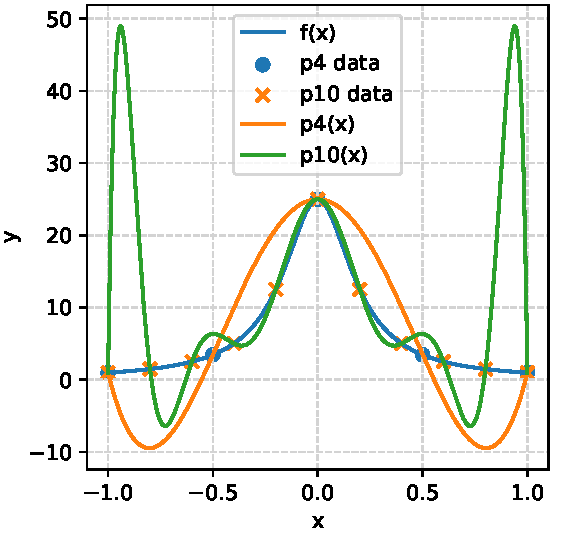
\includegraphics[width=\textwidth]{p4_p10_interpolants.pdf}
\end{columns}
\end{frame}


\begin{frame}
  \frametitle{Final thoughts on polynomial interpolation}
%   \pause
  \begin{itemize}
    \colorize<1> \item An polynomial interpolant of order $n$ requires $n+1$ data points
    \begin{itemize}
     \colorize<1>  \item More data points: interpolant does \emph{not always} cross the points
     \colorize<1>  \item Fewer data points: interpolant is not unique
    \end{itemize}
    \colorize<2> \item Higher-degree polynomials at equidistant points may cause strong oscillatory behaviour (Runge's phenomenon)
    \begin{itemize}
      \colorize<2> \item Mitigation of the problem on Chebyshev (i.e. non uniform grid)...
      \colorize<2> \item ... or by performing piecewise interpolation (next topic)
    \end{itemize}
    \colorize<3> \item Python functions \lstinline$np.polyfit(x,y,n)$ and \lstinline$np.polyval(p,x_new)$ were demonstrated.
  \end{itemize}
\end{frame}

\section{Splines}
\subsection*{}
\againframe<2>{contents_interpolation}
\begin{frame}
  \frametitle{Spline interpolation}
  A spline is a numerical function that represents a {\color{tuealert}smooth}, {\color{tuealert}higher order}, {\color{tuealert}piecewise polynomial} interpolants of a data set.
  \pause
  \begin{itemize}
    \colorize<2> \item Smooth: the interpolant is continuous in the first and second derivatives 
    \colorize<3> \item Higher order: The most common type of splines uses third-order polynomials (cubic splines)
    \colorize<4> \item Piecewise polynomial: The interpolant is constructed between each two consecutive tabulated points
  \end{itemize}
\end{frame}

\begin{frame}
  \frametitle{Splines: comparison to other interpolation techniques}
  \footnotesize\selectfont
  Interpolation of $\displaystyle f(x) = \frac{\sin x}{1+x^2}$
  \begin{center}
    \begin{tikzpicture}
%       \tikzset{at/.style=}
      \begin{axis}[every axis/.append style={font=\tiny},
	width=\textwidth, height=8cm,     % size of the image
	grid = major,
	grid style={dashed, gray!30},
	%xmode=log,log basis x=10,
	%ymode=log,log basis y=10,
	xmin=-4,     % start the diagram at this x-coordinate
	xmax=4,    % end   the diagram at this x-coordinate
	ymin=-0.7,     % start the diagram at this y-coordinate
	ymax=0.7,   % end   the diagram at this y-coordinate
	xtick={-3,-2,...,3},
	xticklabels={ ,-2,-1,...,3}, 
	/pgfplots/ytick={-0.5,0,0.5},
	axis background/.style={fill=white},
	axis x line=middle,
	axis y line=middle,
	ylabel=$f(x)$,
	xlabel=$x$,
	tick align=outside,
	legend style={draw=none,fill=none,font=\tiny,at={(0.5,1.0)},anchor=south},
% 	legend style={pos=outside}
	legend columns=5
	]

	% Actual equation
	\only<1>{\addplot[graph,domain=-4:4] {sin(deg(x))/(1+x*x)};}
	\only<2->{\addplot[graph,domain=-4:4,opacity=0.3] {sin(deg(x))/(1+x*x)};}
	\addlegendentry{Function}
	% Nodes
	\only<2->{\addplot[samples=9,nodes near coords={\color{black}$f_\coordindex$},mark=*,mark options={fill=white,color=tuered},only marks,domain=-4:4] {sin(deg(x))/(1+x*x)};}
	\addlegendentry{Nodes}
	
	% Linear
	\only<3>{\addplot[graph,sharp plot,samples=9,domain=-4:4,draw=tueblue] {sin(deg(x))/(1+x*x)};}
	\only<4-5>{\addplot[graph,sharp plot,samples=9,domain=-4:4,draw=tueblue,opacity=0.3] {sin(deg(x))/(1+x*x)};}
	\addlegendentry{Linear}
	% Polynomial
	\only<4>{\addplot[graph,domain=-4:4,draw=tuegreen] {-6.891773605597105e-04*x^7+2.123474572587917e-02*x^5-2.016362539647688e-01*x^3+6.018261780033977e-01*x};}
	\only<5>{\addplot[graph,domain=-4:4,draw=tuegreen,opacity=0.3] {-6.891773605597105e-04*x^7+2.123474572587917e-02*x^5-2.016362539647688e-01*x^3+6.018261780033977e-01*x};}
	\addlegendentry{Polynomial}
	\only<5>{\addplot[graph,draw=tuefuchsia] table [id=spline]{data/spline_data.txt};}
	\addlegendentry{Spline}
      \end{axis} 
    \end{tikzpicture}
  \end{center}
\end{frame}

\begin{frame}[fragile]
  \frametitle{Spline interpolation in Python}
  We can generate a random data set, and interpolate using \lstinline$scipy.interpolate.interp1d$: 
  \vskip0.5ex \pause
  \begin{lstlisting}[language=Python,basicstyle=\tiny]
import numpy as np
import matplotlib.pyplot as plt
from scipy.interpolate import interp1d
# Generate random data set
x = np.arange(0, 26)
y = np.random.rand(len(x))
# Interpolant on a fine mesh
xc = np.linspace(0, 25, 1001)
yc = interp1d(x, y, kind='cubic')(xc)
# Plot the data
plt.plot(x, y, 'o')
plt.plot(xc, yc, '-r')
  \end{lstlisting} \vskip1ex
        \begin{tikzpicture}
      \begin{axis}[every axis/.append style={font=\footnotesize},
    width=\columnwidth, height=5cm,     % size of the image
    grid = major,
    grid style={dashed, gray!30},
    xmin=0,     % start the diagram at this x-coordinate
    xmax=26,    % end   the diagram at this x-coordinate
    ymin=0,     % start the diagram at this y-coordinate
    ymax=1.3,   % end   the diagram at this y-coordinate
    xtick={0,-2,...,25},
    /pgfplots/ytick={0,0.5,1},
    axis background/.style={fill=white},
    axis x line=middle,
    axis y line=middle,
    ylabel=$f(x)$,
    xlabel=$x$,
    tick align=outside,
    ]

      \addplot[interp,draw=none,mark=*] table [id=spline]{data/spline_data1.txt};
      \addplot[graph] table [id=spline]{data/spline_data2.txt};
    \end{axis} 
  \end{tikzpicture}
\end{frame}

\begin{frame}
  \frametitle{Summary}
  \begin{itemize}
    \item Interpolation is used to obtain data between existing data points
    \begin{itemize}
      \item (Bi-)Linear, polynomial and spline interpolation methods
      \item Construction of Newton polynomials
      \item Oscillations of high-order polynomials
    \end{itemize}
    \item Legendre polynomials: alternative way of performing the polynomial interpolation (not discussed here)
  \end{itemize}
\end{frame}

\section{Tutorials}
\subsection*{Interpolation tutorials}
\begin{frame}[fragile]
  \frametitle{Interpolation tutorials}
  \begin{enumerate}
    \item In Python, generate the data:
    \begin{lstlisting}
x = np.arange(-4, 6, 1)
y = [0, 0, 0, 1, 1, 1, 0, 0, 0, 0]
    \end{lstlisting}
    Interpolate the data using polynomial interpolation (which order do you use?) and a spline. Plot the results together with the original data in a graph.
    \item Do the same exercise for the following data. Can you explain your observations?
    \begin{lstlisting}
t = [0, 0.1, 0.499, 0.5, 0.6, 1.0, 1.4, 1.5, 1.899, 1.9, 2.0]
y = [0, 0.06, 0.17, 0.19, 0.21, 0.26, 0.29, 0.29, 0.30, 0.31, 0.31]
    \end{lstlisting}
  \end{enumerate}
  \textbf{Hint:} Use \href{https://docs.scipy.org/doc/scipy/reference/generated/scipy.interpolate.interp1d.html}{\lstinline{scipy.interpolate.interp1d(...,kind="...")}} to use different splines.
\end{frame}
